\section{Référence et états}
Considérons un solide qui subit une déformation. Celui-ci possède un état initial $\Omega_0$ et un état final $\Omega_t$ 

\begin{figure}[H]
    \centering
    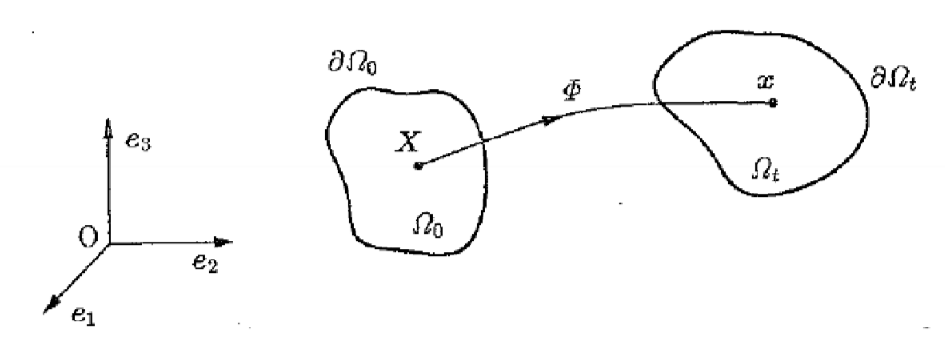
\includegraphics[width = 8cm]{Images/Cinematique/Etats1.png}
    \label{fig:my_label}
\end{figure}
Considérons une particule de ce solide. Son vecteur position est $\mathbf{X}$ dans $\Omega_0$ et $\mathbf{x}$ dans $\Omega_t$.\\
On défini la transformation $\mathbf{\Phi} : \Omega_0 \rightarrow \Omega_t \; \mathbf{X} \rightarrow \mathbf{x} = \mathbf{\Phi}(\textbf{X},t)$

\subsection{Description eulérienne et lagrangienne}

Il existe deux manières de décrire un phénomène en MMC : \\
\begin{itemize}
    \item La description lagrangienne (matérielle) : On place l'observateur sur une particule de matière et on s'intéresse à \textit{comment celle-ci perçoit le champ vectoriel étudié.}\\

    \textit{Exemple : On pose une brindille dans une rivière et on voit comment se déplace la brindille.}\\
    
    \item La description eulérienne (spatiale) : On place l'observateur à un endroit fixe et il observe les particules qui passent sous ses yeux.\\
    
    \textit{Exemple : On donne le champ de vitesse dans un fluide qui s'écoule. En tout point on connaît la vitesse d'une particule.}
\end{itemize}

\subsubsection{Lien entre la description lagrangienne et eulérienne}

\textcolor{red}{Je ne sais pas trop si il faut faire le lien entre les deux description, ou juste évoquer la dérivée langrangienne et l'expliquer (ce que je voulais faire de base)}

Si on étudie une grandeur avec une description lagrangienne, il faut faire attention en la dérivant. Considérons la grandeur $\mathbf{K}(\mathbf{X}, t)$, calculons sa dérivée temporelle.
\begin{equation*}
    \frac{\partial}{\partial t} \mathbf{K}(\mathbf{X}, t) = \frac{\partial \mathbf{k}}{\partial t} + \frac{\partial \mathbf{k}}{\partial \mathbf{x}} \frac{\partial  \mathbf{x}}{\partial t} = \frac{\partial \mathbf{k}}{\partial t} + \underbrace{\frac{\partial \mathbf{k}}{\partial \mathbf{x}}}_{\nabla \mathbf{k}} \mathbf{v}(\mathbf{x}, t) \equiv \frac{\mathcal{D} k}{\mathcal{D} t}
\end{equation*}

\textcolor{red}{Je suis peut être le seul à avoir galéré à comprendre ça (l'interprétation physique), du coup dites moi si c'est pertinent ou non, auquel cas on peut l'enlever. (Julien Monfils)}\\

\textit{Interprétation physique :}
\\

\textit{
Plaçons un observateur sur une particule traversant un champ de température qui ne varie pas dans le temps} $(\frac{\partial k}{\partial t} = \frac{\partial T}{\partial t} = 0)$.\\

%Y a une erreur Latex ici, jsp pourquoi
\textit{On s'intéresse maintenant à la dérivée de la température mesurée par l'observateur. Selon la formule développée ci-dessus, on a}
\begin{equation*}
    \frac{\mathcal{D} T}{\mathcal{D} t} = \nabla T \cdot \mathbf{v}(\mathbf{x}, t)
\end{equation*}
\textit{La relation de proportionnalité entre la dérivée temporelle de $T$ et la vitesse de la particule peut s'expliquer de la manière suivante :}\\

\textit{Si l'observateur ne se déplace pas dans le champs de température, il ne perçoit aucune variation de température, la dérivée temporelle est donc nulle.}\\

\textit{Si l'observateur est mobile, la dérivée temporelle sera proportionnelle à la vitesse. En effet, plus il se déplacera vite, plus les changements de températures qu'il percevra seront rapides.}

\section{Gradient de déformation}